\chapter{Implementation}
The tool has now been used in a practical example to give an idea of how it is used to enhance the development experience.
This chapter will go into the design decisions and implementation details to make each part and feature of the tool function, as well as,
explain what the tool consists of and how the components work together to create the finished product.

The specifics of the code will be omitted, but the general control flow of each part of the tool will be explained.

\section{Overview of the Components}
The tool essentially consists of four components: The VS Code extension, the user interface written in Svelte, the \javatoolname[] program written in Java and an adapter program for \javatoolname[] which uses NodeJS called \nodetoolname[].
The \javatoolname[] program is used to run the Jolie parser, which is also written in Java, and that will gather all information from the Jolie code needed by the visualization tool.

The Svelte user interface is the component which takes in the user input and renders the services, ports and connections.
In order for the UI to get the relevant data from the Jolie code, the VS Code extension invokes the \nodetoolname[], with the correct parameters, which invokes the \javatoolname[] program.
\nodetoolname[] listens for the output of the \javatoolname[] program,
meaning that the \nodetoolname[] functions as a wrapper for the \javatoolname[] program so the VS Code extension does not have to invoke \javatoolname[] directly,
and sends the data to the VS Code extension, which sends the data to the user interface.

\cref{figure:comp_diagram} displays the connection between the different components.

\begin{figure}[t]
    \center
    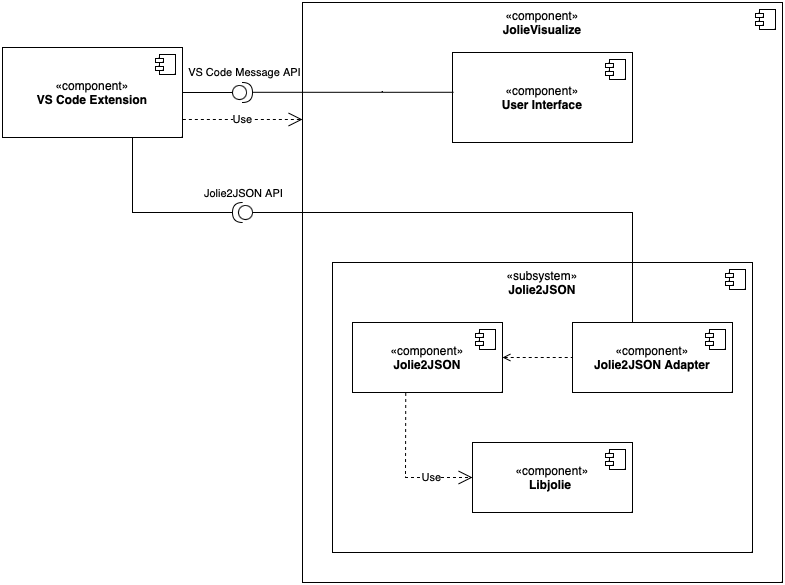
\includegraphics[width=0.80\textwidth]{figures/component_diagram.png}
    \caption{A diagram of the different components of the tools. The JolieVisualize tool contains the user interface and the Jolie2JSON subsystem which includes the adapter for the VS Code to communicate with the parsing program.}
    \label{figure:comp_diagram}
\end{figure}

\section{Data Representation}
The data which the \javatoolname[] program will output is consistent through all
four components of the tool. The chosen data format is JSON data because it is easy to parse in TypeScript, which most components use.
The data needed for the tool is a list of interfaces, a list of types and the list of services.

\subsection{Interfaces \& Types}
Each interface in the list of interfaces has a name, identifier, file path, and two lists of operations.
One of the lists contains all one-way operations, and the other contains all request-response operations.
The request-response operations consist of the operation name, the request type name and file path pair and the response type name and file path pair, and for one-way operations it is similar but with the response type omitted.

Having the type name and file path pair as a separate type object list instead of the type object directly in the specific interface object is a design decision made at the very start of the development process.
Each interface could have a list of types which will save computation when the user clicks on the type in the sidebar and the type is displayed because only the interface's list of types needs to be searched for the correct type.
This, however, has the drawback of a lot of duplication, only if all interfaces in the system use a unique set of types can this issue be avoided.
This is why a global list of types is used. The interfaces then reference what types are used for operation and the global list of types can be used when using the sidebar to view interfaces and types, and by
using the Jolie language constraint of no duplicate type names in the same OL file, the file path and type name are enough to find the correct type when searching for it.

The list of types, as mentioned, contains all types used by all interfaces in the architecture.
Each type object in the list represents the information about a type in the code, this includes the name of the type, the file in which the type is defined, the root type, subtypes which is a list of types as well, and cardinality of the type in case of this being defined.
If the type is a \textit{choice type}, the two choices are also represented in the type object as strings which reference other types in the global list.\footnote{Types in Jolie - \url{https://docs.jolie-lang.org/v1.10.x/language-tools-and-standard-library/basics/data-types/index.html}}
Types from \textit{interface extenders} are also added to this list.

An example of the JSON data used to represent interfaces and types from Jolie can be seen in \cref{appen:joliejson_iface_types}.

\subsection{Services \& Networks}
The last list in the global JSON is the list of services. The list of services is also used to infer how the networks are set up and which services reside in each network.
This approach draws inspiration from how bigraphs are used to model software architecture. Bigraphs are a type of graph consisting of two sub-graph components. The link graph and the place graph. The link graph models the connection between nodes in the system while the place graph models the topology.
The nodes in the system of the bigraph can be directly mapped to Jolie services. Bigraphs also model ports which are a component of Jolie services as well.
The data representation used for the tool draws the most inspiration from the place graph since the link graph is inferred by the locations and protocols of the ports in Jolie.
A place graph models the topology and the networks, which are called \textit{roots} in bigraph terminology, and also embeddings, which are called \textit{nestings}.
The bigraph inspiration is taken from \textit{The Space and Motion of Communicating Agents} by Robin Milner \cite{BigraphBook}, where bigraphs are formally introduced and explained but are not necessary for this use-case.

The place graph component can be seen as a list of trees where the root is the network and contains all top-level services as immediate children and embeddings of the top-level services are the children of those services.
This fits well with how a Jolie system can be modelled, so the list of services in the global JSON is essentially a place graph or a list of trees where each node is a service in the system.
Each root in the list of trees is a network. In the sense of JSON, the network is a list of services since it can have any number of children, and the \textit{embeddings} list of each service is also a list of services.

The services in the JSON also need to contain all other information which is used by the tool.
This includes the input and output ports, execution target, name, identifier, and file path but also the information specified in the architecture file, which is container name, volumes, parameters etc.

An example of the JSON data used to represent services and ports from Jolie can be seen in \cref{appen:joliejson_services}.

\subsection{Architectural Programming}
The architectural programming features in Jolie also need to be represented in the data to visualize it in the tool's UI.
This includes couriers, collections, aggregations, and redirections. The information is represented in the ports of the JSON since the features are port specific and are either created in ports or reference ports in the code.

Aggregations in the JSON are represented by the name of the output port to aggregate to, optionally the aggregate can have an interface extender which is defined here.
Collections are essentially a list of aggregations, so collections are also represented in the aggregates as a list of names of the output ports, and because multiple output ports of one service cannot have identical names, this will not create ambiguity.

Couriers are defined in Jolie based on an input port with aggregation, so the port also represents the couriers of that port.
The couriers in the JSON have lists of operation names and interface names which the courier will act upon. This is both for request-response and one-way operations and for whole interfaces. The names refer to the operations and interfaces in the system.

Redirections for an input port are a list of pairs of resource and output port names. This represents how a resource is redirected to an output port.
However, since the resource of the redirect is defined using the location of the output port, the output port will not be connected correctly unless the resource part of the string is removed, so the resource part of the location, namely,
the part after \texttt{/!/} is removed and placed in a separate field in the JSON for the output ports.

All types of architectural programming features in the JSON representation of Jolie can be seen in \cref{appen:joliejson_architecture}.

\subsection{Prototype Data}
The data used to create the prototype is also represented in JSON and is split into two parts, the Docker-Compose YAML file content and the service folders which contain the Jolie files, dependencies, and Dockerfile.
The Docker-Compose file content is simply a string, which will be written to the file. The service folders are used to generate this string, but this will be explained more in detail in a later section.
The services folders, which are called build folders internally, are an array of objects that each represent a folder to be created when generating the prototype.
The build folders have to represent what a Docker image will contain, so each folder can be seen as a Docker image. This has to be independent of the Jolie code since two identical services can have different parameters or runtime arguments which means that they should be two different images.

Each build folder contains a list of files which will be added to the folder itself, but also a list of files which will be added to the shared resource folder.
Information such as runtime arguments, exposed Docker ports, and the service name is also added to the build folder JSON because the Dockerfile needs this information when it is being generated.

The JSON data generated to create the prototype can be seen in \cref{appen:joliejson_prototype}, but with omitted docker-compose YAML content.

\section{The \nodetoolname[]}
% why it is created and how it works
The \nodetoolname[] functions as a wrapper for the \javatoolname[] program. It is created so the VS Code application does not have to execute the \javatoolname[] program directly and also if the tool should be extended to other code editors or run in the browser, this functionality should not be implemented in the VS Code extension.
The \nodetoolname[] also makes sure to return errors if a parsing error occurs or if Jolie is not installed correctly.

This part of the tool consists of three parts, the data fetching part which executes the \javatoolname[] program and checks for errors, the server part which allows the developer to visualize their program's architecture directly in the browser but without the code refactoring functionality, and
prototyping which is identical to the functionality in the VS Code extension, but this can be used if the user of the tool installs only this part of the tool without the VS Code extension.
The server uses the express framework\footnote{Express Framework - \url{https://expressjs.com/}} to open an endpoint to get the JSON data and also serve the webpage as static assets on localhost.

\section{The \javatoolname[] Program}
% how the data is fetched in the Java tool
The \javatoolname[] program is written in Java and is used to gather the required information from the Jolie code. The Jolie parser is written in Java and therefore the \javatoolname[] program here uses the parser directly to get the abstract syntax tree nodes and create the JSON objects.

The \javatoolname[] program has two types of outputs which is used by the tool. The JSON representation of the entire system and the information used by the prototyping functionality. Both functionalities of the \javatoolname[] program require the whole system to be parsed using the Jolie parser.
Firstly, the tool creates the networks by parsing the architecture JSON file and making an internal representation of what it contains. The networks contain a map of top-level services mapped to a \texttt{ServiceNode} which is the abstract syntax tree (AST) node of a service from the Jolie parser. The top-level service is a representation of a Jolie service in the architecture file, as seen in \cref{appen:architecture-file-structure}.

The \javatoolname[] program uses a lightweight JSON library, \textit{json-simple}, to parse files and create JSON objects\footnote{JSON-simple - \url{https://code.google.com/archive/p/json-simple/}}.
To get the ServiceNode AST node from the parser, the Jolie parser is invoked using its module parsing method. This returns the whole AST of a file, called a \textit{program}. All ServiceNodes are then captured and added to the network's map object.

When the networks have been created, depending on if the program should send visualization data or prototyping data, all the necessary information about the services, ports, etc. is created.
\subsection{Parsing the Jolie System}
A system inspector has been created in order to parse the networks.
The system inspector uses the created list of networks containing the top-level services and ServiceNodes.
The inspector goes through each network's map object and creates a service object which is an internal representation of the services used by the tool.
It creates the services by looking at all the child nodes of the ServiceNode AST node in a loop and using type comparison to check what child node is being looked at and how to parse the information correctly.
Relevant child nodes for a service are: \textit{ExecutionInfo}, \textit{CourierDefinitionNodes}, \textit{EmbedServiceNodes}, \textit{InputPortInfo}, and \textit{OutputPortInfo} nodes.

Service objects can also have a list of services which are considered embeddings. When looping through the AST nodes of a service, embedded service nodes will be used to create services, which are added to the parent's list of services instead of the global list of services.
This will enforce the place graph structure of services mentioned in the data representation section.

The most complex of the child nodes are the two types of port nodes. Input and output ports also have an internal representation in the \javatoolname[] program which keeps track of all the necessary information about the ports used by the tool.
Ports have to contain information about the location, protocol, name, interfaces and operations.
When the ports are being created, the interfaces which are used by the ports will also be created. These interfaces are also represented internally and will store information about the operations.
The operations are also parsed using type comparison, since two types of operation declaration AST nodes exist in Jolie, namely, request-response and one-way.
The interfaces are added to a global object \textit{JolieSystem} which has information about all parsed services, interfaces and types.

For input ports specifically, information about aggregates, collections, couriers and redirects is also stored. Redirects can be seen as a mapping where a resource is mapped to a port name. This is how the Jolie parser represents redirects as well, so this is simply copied over to the tool's representation.
Aggregates are simply a name of an output port but can contain collections and interface extenders, however, Jolie's internal representation of aggregates contains this information so the interface extender just has to be created to match the tool's representation of interfaces, and collections are a list of output ports which will be copied directly.

When the interfaces are created the types used in the operations are also parsed and created in an internal representation.
This representation stores information about the root type, cardinality, subtypes, etc.
The types in Jolie can also be three different AST node types, namely definition links, inline definitions and choice definitions. Type comparison is also used here to parse the type correctly depending on the AST node type.
Types are, similarly to interfaces, added to the system's global list of types.

Each building block of a Jolie service has an internal representation in the \javatoolname[] program and all of them have a \texttt{toJSON} method which takes all information stored in the objects and creates a JSON object.
When the tool invokes the \javatoolname[] program to get the JSON data, the \texttt{getJSON} method is invoked on the global JolieSystem object which cascades and invokes the getJSON method for all internal objects which also carcades to its internal objects.
This will result in a JSON object which resembles the data representation discussed in the previous section, and this JSON can be used by the other components of the tool.

\subsection{Generating the Prototype Data}
The \javatoolname[] also creates data for making the prototype. This includes the content of the Docker-Compose YAML file and the information needed for creating the service folders and the resource folder.
After the whole system has been parsed and a JolieSystem is created, the system will be given as a parameter to a \textit{build} object which will handle the logic for creating the JSON data.
The builder will first create the service folders using the services in the networks from the JolieSystem object. Duplicate build folders will be checked for at this stage, which is done to make sure that duplicate images will not be generated when using Docker-Compose.
However, as mentioned in a previous section, two identical services can be two different images if, for example, the runtime arguments are different. This is also handled here.
The build folders contain a list of files which are needed for the service to run. This is essentially the file in which the target service resides and all dependency files.
To get all the dependencies of a service, the service representation in the system inspector has a set of strings corresponding to the file URIs of the imported symbols.
When the inspector goes through embeddings, types, interfaces, etc, of a service it adds all file URIs to the set which can be used to make the list of dependencies when creating the build folder.

After the build folders have been created as internal objects, they are parsed onto another object which builds the Docker-Compose YAML string. The JolieSystem is also used here to create the networks in the Docker-Compose file.
The Docker-Compose builder also has some internal representation of what a service is, since two services in Docker-Compose can use the same image but have different deployment properties, which means that they should be created as separate services in Docker-Compose, but they will not have two different service folders.
The Docker-Compose builder uses a string builder to create the YAML file content. It goes through all services and creates an internal \textit{compose service} and like with the service folders, composes duplicates and counts replicas.

The networks are also created in the Docker-Compose YAML, which can have another semantic meaning from the networks defined in the architecture file.
In Docker-Compose networks are used to restrict services connecting, which is not a problem with a system created in Jolie, so to have the Docker-Compose networks work similarly to how networks in the tool work, each service in Docker-Compose is set to be a part of
its network, as specified in the architecture file, but also all other networks that the service has a port connecting to.\footnote{Networks in Docker-Compose - \url{https://docs.docker.com/compose/networking/}}

\section{Visualization User Interface}
After the JSON data has been created using the \javatoolname[], it needs to be rendered in a user interface, which can handle user input as well.
There are two aspects of these components, firstly, how to create a reactive user interface which can handle user input and handle updates based on how the user interacts with the tool. Secondly, how the components of the architecture are rendered efficiently and how they should be laid out to make the architecture comprehensible and manageable.

\subsection{User Interface}
The tool's user interface is essentially a static webpage where the JSON data is loaded when the site is initialized.
The UI uses CSS for styling and JavaScript for the logic, like most standard websites.

However, creating a very feature-heavy reactive user interface in standard CSS and JavaScript is almost impossible in a reasonable amount of time.
The first improvement to the development of the UI was to replace JavaScript with TypeScript (TS).
TS is a transpiled and typed programming language, created by Microsoft, which is a superset of JavaScript. It compiles directly to JavaScript which makes it usable by the UI webpage.
Some of the benefits of using TS include type checking, self-documenting code, interfaces, and generally enhanced productivity.\footnote{TypeScript - \url{https://www.typescriptlang.org/}}

Writing standard CSS can also be a very tedious process, so to enhance the development experience TailwindCSS, or just Tailwind, is used.
Tailwind is a CSS framework which aims to move CSS to the HTML components. CSS properties are defined in the class attributes of the HTML components where readable class names have been defined meaning that any combination of these classes can be used to style components.
Tailwind also defines a design system which a developer can use to enforce a standard when it comes to the design of the UI, and with tools like \textit{postcss} and \textit{autoprefixer} the build size of the utility CSS components will be kept at a minimum.\footnote{TailwindCSS - \url{https://tailwindcss.com/}}

\subsection{Rendering \& Layout}
All services, ports and edges between ports are rendered using SVG components.
Different SVG\footnote{SVG Elements - \url{https://developer.mozilla.org/en-US/docs/Web/SVG}} elements are used for different parts of the UI. Polygons are used to render service shapes, rectangles are used to render ports and paths are used to render edges between ports.
SVG elements in HTML are easy to manipulate in TS, so when the JSON data is loaded in, the correct HTML components are created and then TS is used to create the SVG data for each component so they get the desired shape and size.
To help with the manipulation of SVG elements in TS, a library is used called \textit{D3.js}.\footnote{D3.JS - \url{https://d3js.org/}} D3 has a long list of features to help visualize data using SVGs, however, the only functionality used for this tool is
the ability to select SVG components and apply attributes, event handlers, and stylings.

The problem with D3 is that it has no way of doing the layout of the services and ports.
To ensure that the architecture is always readable from the UI, and the connections of ports are visualized practically, a framework/library is used.
The framework needs to support the visualization of embeddings, networks and connections between ports.

Different frameworks were tested to see which gave the best results while providing the capabilities needed for the tool.
The first framework tested was MermaidJS\footnote{MermaidJS diagramming tool - \url{https://mermaid.js.org}} which is a diagramming and charting tool. Mermaid uses markdown to represent components in a diagram and does the rendering and layout of the components. Using this tool would mean that D3 was no longer necessary, however, MermaidJS uses D3 internally for the rendering along with Dagre-D3\footnote{Dagre-D3 - \url{https://github.com/dagrejs/dagre-d3}} for layout.
The problem with MermaidJS is that it is not generic enough, it supports rendering and layout for a long list of specific diagram types, but none of the types would fit the rendering of services in a microservice architecture.
MermaidJS can draw simple graphs which could work as a foundation for the tool, but this is wasteful. The framework has a lot of capabilities which would go unused.

As mentioned, MermaidJS uses Dagre-D3 for the layout of components, which is the next framework tried for the tool.
Dagre is a graph layout library which primarily focuses on the layout of directed graphs. Dagre-D3 provides rendering using D3 on top of the base Dagre library.
Dagre and Dagre-D3 are both deprecated libraries, even though it is still used by many including MermaidJS.
The problem with Dagre-D3 is that the scope of the library is directed graphs, and nothing more.
Embeddings are not possible to represent.
It is possible to have \textit{Clusters}\footnote{Dagre-D3 clusters - \url{https://dagrejs.github.io/project/dagre-d3/latest/demo/clusters.html}}
but the clusters work more like a grouping of vertices in a graph and not like a vertex having vertices inside it, which is essentially how the embeddings should be represented if a graph library is to be used.

Another library that was also tried but has many of the same drawbacks as Dagre-D3 and MermaidJS is Cytoscape.\footnote{CytoscapeJS - \url{https://js.cytoscape.org}}
This library is also a graph visualization and layout library. It comes with a lot of features out of the box like animations and dragging of the vertices. The main issue of this library is that embeddings are
not possible, but also that many of the built-in features do not fit the visualization tool.

The framework that was chosen for the tool is Eclipse Layout Kernel (ELK)\footnote{Eclipse Layout Kernel - \url{https://www.eclipse.org/elk/}}
which is a layout framework with a collection of different layout algorithms. The tools currently use the layered layout algorithm which is based on \textit{Methods for Visual Understanding of Hierarchical System Structures} by Sugiyama, Tagawa and Toda.\cite{4308636} ELK supports embeddings, ports and edges. This is essentially everything the tool needs for the layout capabilities.
ELK only does layout, however, so the rendering needs to be done by a separate library, where D3 is chosen to render the components of the architecture when ELK has done the layout.
\cref{figure:elk_example} shows a system being laid out using ELK.

\begin{figure}[h!]
    \center
    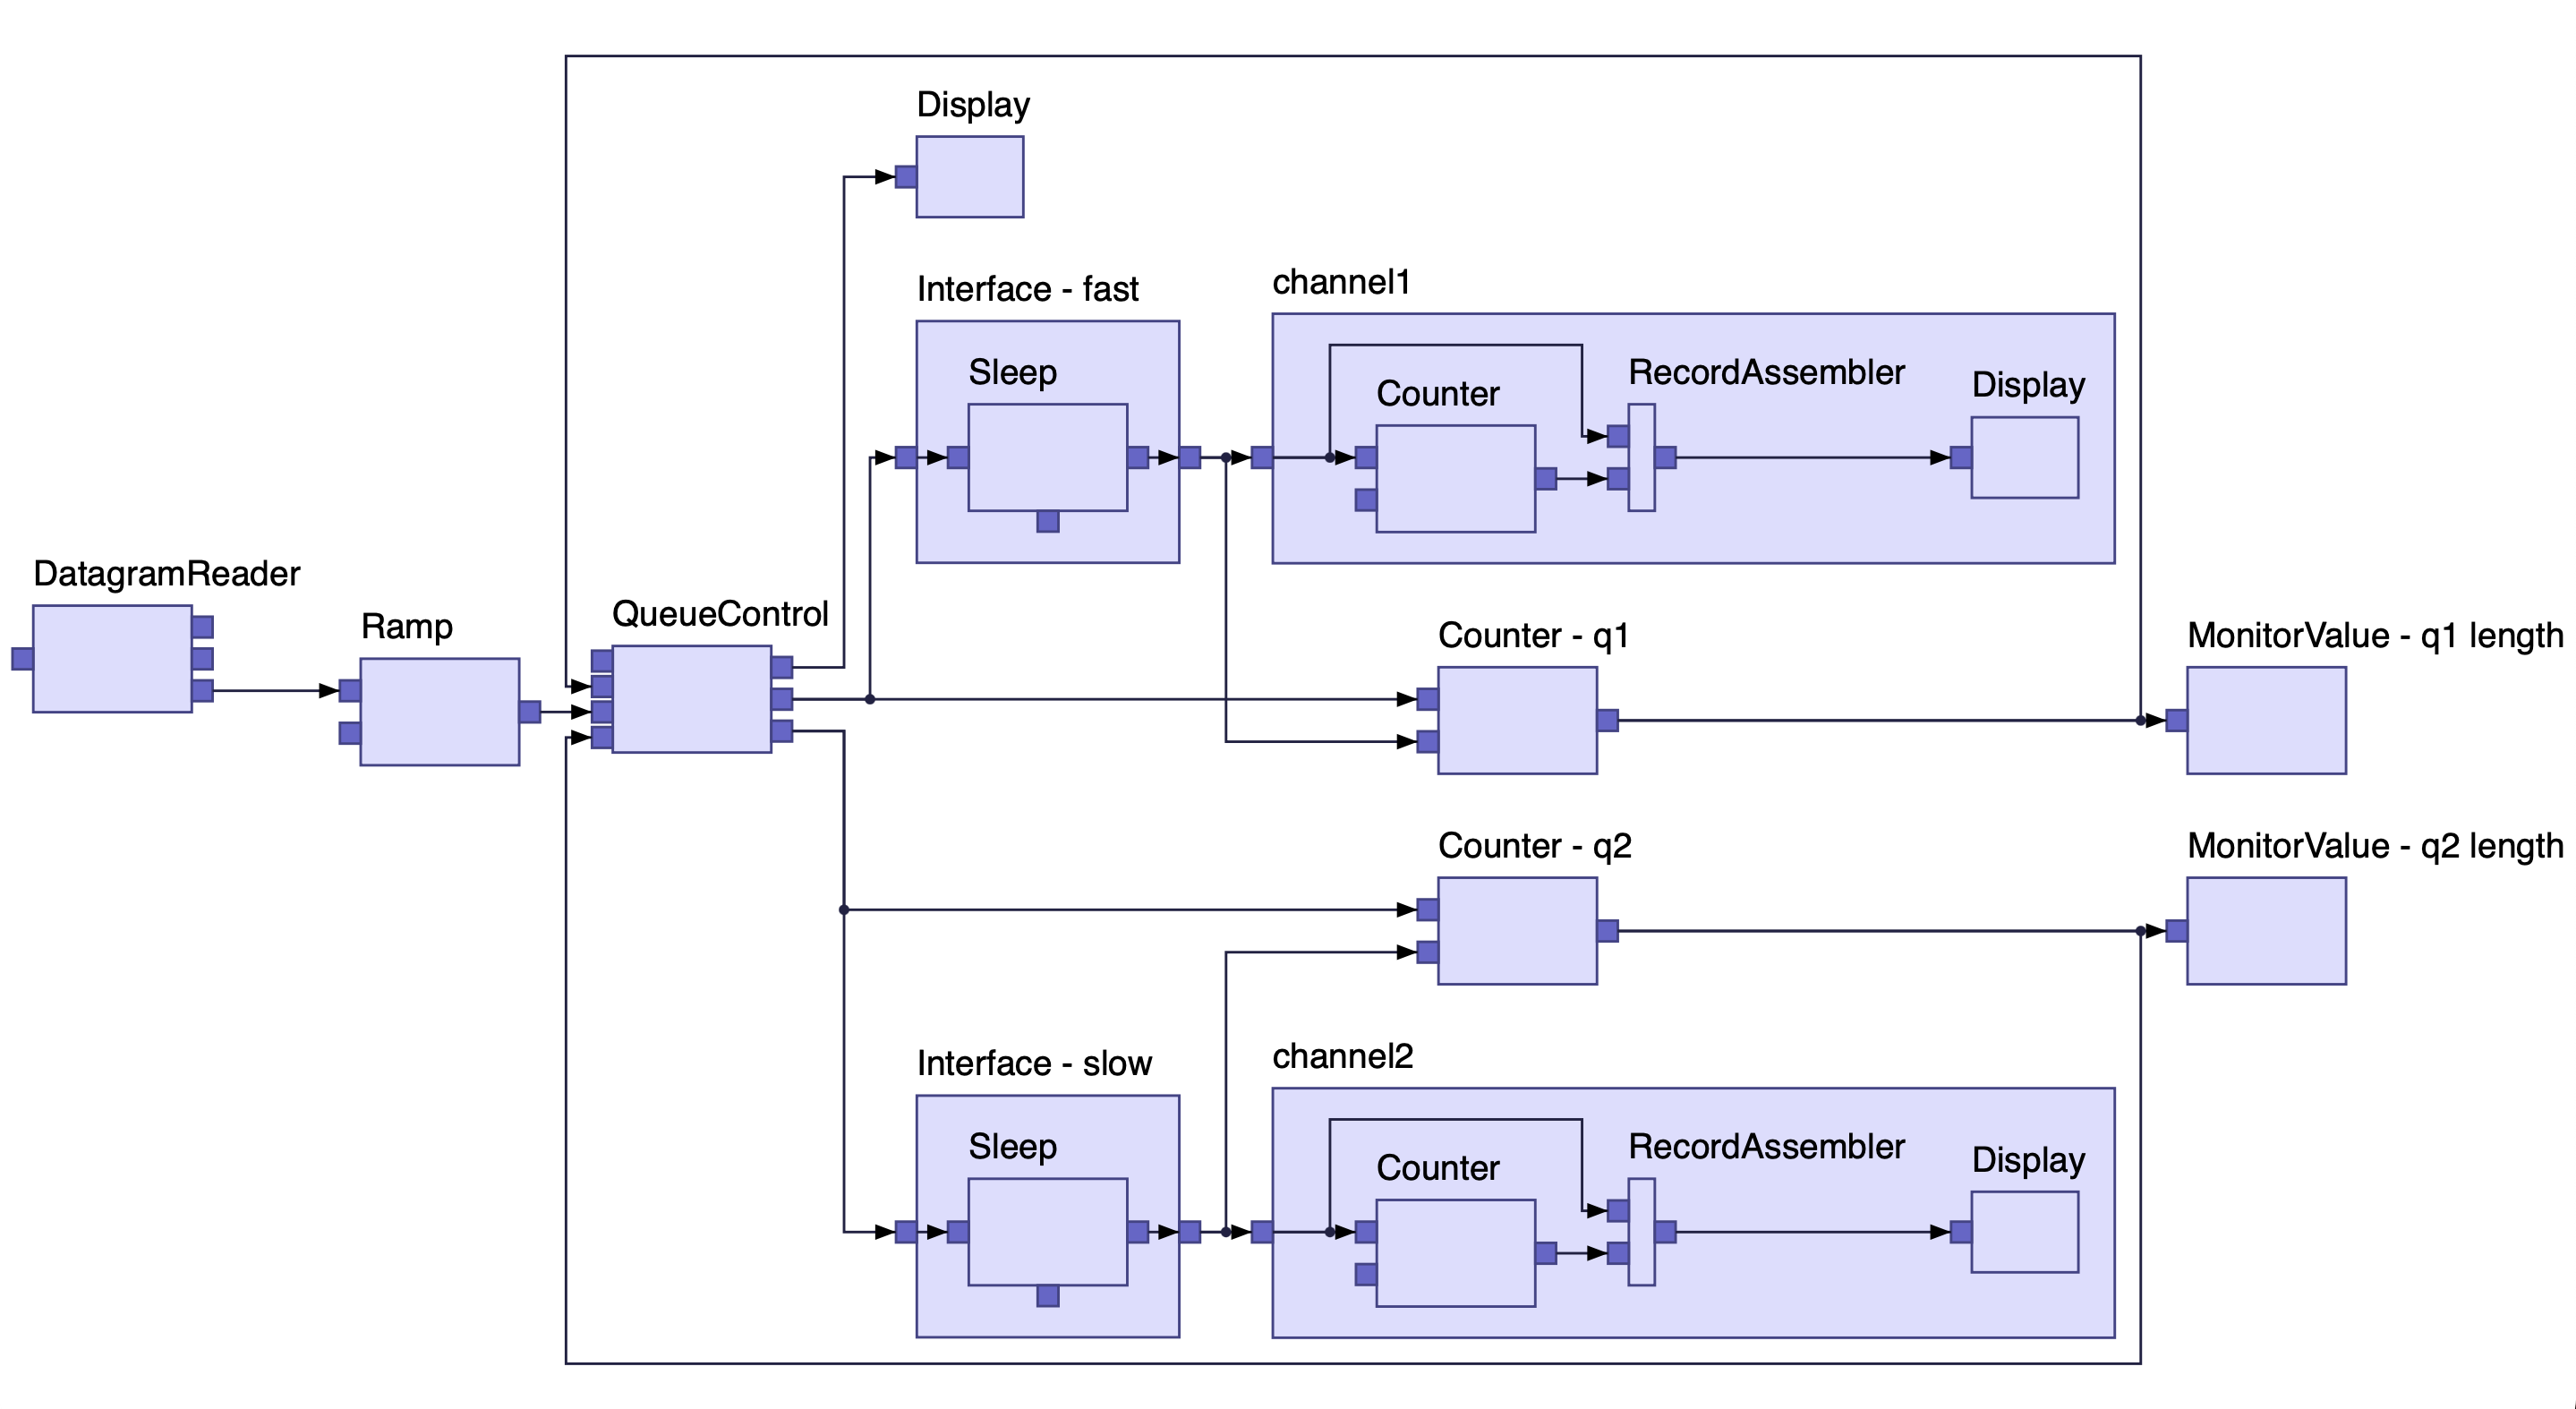
\includegraphics[width=0.80\textwidth]{figures/elk.png}
    \caption{A system using ELK to layout each component of the system including ports and embeddings. Connections between ports are also calculated. The rendering of the system is not done using ELK. Source: \url{https://www.eclipse.org/elk/img/example_layout_complexRouter.svg}}
    \label{figure:elk_example}
\end{figure}

The drawback of using ELK is that in a highly reactive UI, the user might want to position the services themselves, which is not yet possible with ELK.
So when the components of the architecture have been positioned in a network, for example, a service cannot be positioned inside the network. It can however be moved outside the network to move it to another network.
The drawbacks of using ELK do not outweigh the benefits. Having direct support for ports and embeddings is very valuable for the tool, and that is why it has been chosen as the layout framework.

ELK has a TypeScript version, so it can easily be used with the rest of the user interface. To make ELK calculate the layout of the JSON data from \javatoolname[] it needs to be converted into a format which ELK understands.
ELK has a textual graph DSL but also supports a specific JSON format, which is used by the tool because of simple conversion. This format can be seen in \cref{lst:elk_json}.

\begin{jsonlisting}[][caption={The ELK JSON format}, label={lst:elk_json}]
{
    "id": "root",
    "layoutOptions": { "algorithm": "layered" },
    "children": [
        { "id": "n1", "width": 30, "height": 30 },
        { "id": "n2", "width": 30, "height": 30 },
        {
            "id": "n3",
            "width": 30,
            "height": 30,
            "ports": [
                { "id": "p1", "width": 5, "height": 5 },
                { "id": "p1", "width": 5, "height": 5 }
            ]
        }
    ],
    "edges": [
        { "id": "e1", "sources": [ "n1" ], "targets": [ "n2" ] },
        { "id": "e2", "sources": [ "n1" ], "targets": [ "n3" ] }
    ]
}
\end{jsonlisting}

When the UI receives the JSON data containing the networks with services, the ELK graph is created based on the JSON data.
The networks are the children of the root node of the ELK graph. This is specified in the \texttt{"children"} field of the ELK JSON.
ELK nodes in the graph have a field for ports, which are positioned around the node when the layout algorithm is invoked.

To connect the ports with edges, edge objects can be added to the ELK nodes. Embedded connections will be placed in the parent's edge list in the ELK graph, and inter-service connections will have edges in the network containing the services.
Multiple local output ports are handled so the UI can differentiate between local output ports when embedding and disembedding services to avoid removing unwanted ports or rendering connections between ports which should not be there.
This is done in a preprocessing step when the UI gets the Jolie system JSON, where local input ports will be matched to the corresponding output port of the embedder and the location will be unique between the two ports to remove ambiguity.
Connections that are happening between networks are placed at the root of the ELK graph. To determine what edges should be added to the graph, all output ports will be checked to see if a matching input port exists anywhere.

When the ELK graph has been populated with the necessary nodes and edges, the layout is calculated. All the components of the graph get a position and size, and all edges get a list of points. D3 can then render the graph components.
The ELK JSON represents what is rendered in the UI, so embeddings of the top-level services are not added to the ELK graph. When the user of the tool expands a service the embedded services will be added to the ELK graph and
everything gets recalculated and then they are re-rendered correctly in the UI. Generally, every time the user does something in the UI which requires the ELK graph to be modified, the layout algorithm is run.

\subsection{UI Framework}
To facilitate the reactivity needed for the UI when the user starts manipulating the architecture, a UI framework called \textit{Svelte}\footnote{Svelte - \url{https://svelte.dev/}} is used.
Svelte is a framework used to create reactive web interfaces similar to React, Angular, and Vue. The benefit of using Svelte instead of any of the other frameworks mentioned is that Svelte compiles into highly efficient JavaScript,
whereas most of the other frameworks ship some sort of DOM manipulation engine alongside the code. Svelte is the chosen framework because it must run in VS Code which runs in Electron\footnote{Electronjs - \url{https://www.electronjs.org/}}, and the speed is a factor in this case.

Svelte is component-based and works by combining stylings, markup and JavaScript/TypeScript into one file type. Svelte allows the injection of JS variables into the markup, and updating the variables will force a redrawing of the DOM, which makes the user interface reactive.
The user interface is composed of a component tree where the "app" component is the root which holds information about the current ELK graph. \cref{figure:component_tree} shows the component tree of the user interface. The sidebar and popup window are child components of the root app component, meaning when they are updated, the DOM is re-rendered. 
The parent component also contains the SVG parent component which holds all component shapes of the system.
The ELK graph is used here to create network child components. The network components take in the corresponding subgraph as input, which the network can use to create the service and edge child components.
The service components also have edge components which represent the internal edges which connect output ports to the input ports of embedded services.
The zoom component which handles the scaling and transposition of the SVG is also added to the root component to enhance user experience.

All components in Svelte have lifecycles which are utilized to render the components with D3.js.
The lifecycle loop consists of four stages where all of which have event handlers directly accessible in the TypeScript code in Svelte files. This means that each component can run code at any stage of its lifecycle.
The four events are: \textit{before update}, \textit{on mount}, \textit{after update}, and \textit{on destroy}.
\textit{Before update} happens before anything else. It runs every time the component is updated and before the DOM is created.
\textit{On mount} runs only once when the component is created and runs right after the DOM is created. 
\textit{After update} runs after the DOM is created and runs every time the component is updated.
Lastly, \textit{On Destroy} runs once when the component is destroyed.\footnote{Svelte lifecycle functions - \url{https://svelte.dev/docs\#run-time-svelte}}
All components of the graph will have position and size when they are created because ELK has done the layout at that point.
So when creating the DOM elements for each component, the size and position are already known.
Components which are rendered with D3 have an "after update" event handler which will run \textit{after} the DOM for the component is created. This code uses D3 to render the desired shapes.

The \textit{before update} event handler is used to map the ELK graph component to an object from the Jolie system JSON, because it runs before the DOM is created, it can be used to check if a service component is expanded or not, which allows the DOM of the service to change.

The whole component tree does not re-render if a service is changed by the user. Only when the ELK graph in the root component is updated, will the whole component tree be re-rendered. To make sure that the ELK graph is updated when a service or port is changed, an event dispatcher is used to 
send events up the component tree. Ports and services can send events which their parents listen for and will aggregate towards the root. When the root gets a specific event, it will trigger the ELK layout algorithm and re-render the whole component tree.

The last Svelte-specific concept used is \textit{stores}.\footnote{Svelte stores - \url{https://svelte.dev/docs\#run-time-svelte-store}} Stores in Svelte are global states which can be used by all components of the program. Stores can be written to, which overwrites the object saved in the store, and they can be subscribed to by components which will run some code every time a store is changed.
In this UI, stores are used to keep a state of what is displayed in the sidebar and popup window. This allows all components of the application to write to the store and determine what is displayed in the sidebar or the popup window. 

\begin{figure}[t]
    \center
    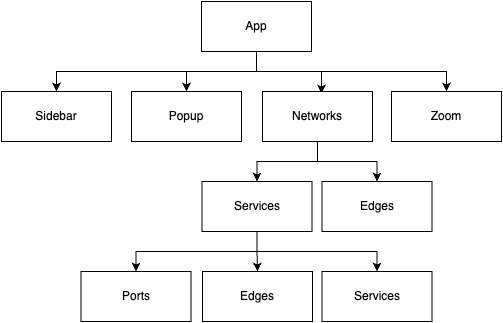
\includegraphics[width=0.70\textwidth]{figures/component_tree.png}
    \caption{The component tree of the user interface created in Svelte. When the root component is updated an update is cascaded down the component tree.}
    \label{figure:component_tree}
\end{figure}

\section{Visual Studio Code Extension}
The VS Code extension generally consists of the activation events, contribution points and a web view.
The activation events determine what will activate the extension. An example could be that would be when a certain file type is opened, the plugin is activated.
For this extension, the activation events happen by commands which the user can type into VS Code. The commands are displayed in \cref{appen:vscode_commands}.

The contribution points\footnote{Contribution Points in VS Code - \url{https://code.visualstudio.com/api/references/contribution-points}} are declarations of enhancement that the extension does. There is a long list of different functionalities which can be extended.
This extension's contribution points only include snippets. The snippets are used when creating the architecture file. The snippets work by suggesting auto-completion in JSON files, where the user can press the tab key to jump to different points in the inserted code to quickly edit.
The list of snippets from this plugin can be seen in \cref{appen:vscode_snippets}.

The last overall part is the web view that VS Code facilitates.\footnote{Webviews - \url{https://code.visualstudio.com/api/extension-guides/webview\#scripts-and-message-passing}} The web view can be used to fully render web content in the editor.
This can be seen as an iframe within VS Code. When the web view is created custom HTML can be set. This HTML can reference JavaScript and CSS code from the host machine's local resources, meaning that the compiled JavaScript and CSS from the user interface made in Svelte, can be used directly in the VS Code extension web view.
This is done by having the extension install the JolieVisualize node package and referencing the compiled Svelte code in the \texttt{node\_modules} folder.

The extension can send messages to the web view using a post message function which sends serializable JSON data to the web view.
The JavaScript running in the web view can create an event listener which listens for messages. The payload of the messages declares what type of message is sent and then the web view can act accordingly.
This is useful when the UI should update based on some event in the editor.

\subsection{The VS Code API \& Commands}
VS Code exposes an API\footnote{VS Code API - \url{https://code.visualstudio.com/api/references/vscode-api}} with a long list of operations and events
which is used in this extension to handle all inputs from the UI, and the code editor.
The API is split into different namespaces where this extension primarily uses the \texttt{workspace}
namespace. This includes all operations and events regarding folders and files in the working directory.
Specific events and operations will be explained more in detail when discussing their applications in this extension.

The built-in commands\footnote{VS Code Commands - \url{https://code.visualstudio.com/api/references/commands}} which VS Code provides can be programmatically executed.
Many of the commands use \textit{providers} to define how they are implemented. This means that the commands essentially execute a provider which can be implemented by the language server protocol (LSP).\footnote{Language Server Protocol - \url{https://microsoft.github.io/language-server-protocol/}}
Providers can also be implemented in the extension or any other extension.
This is useful because the extension can invoke LSP functions programmatically. How the LSP can be utilized for this tool will be discussed in a later section.

\subsection{Live Updates}
When the user of the tool changes something in the code while the tool is running, the visualization UI automatically reflects the changes done in the code.
Two event listeners are used to keep the UI up-to-date with the code when a change happens in the code. \texttt{OnWillSave} and \texttt{OnSave}.
\texttt{OnWillSave} is an event which fires when the user saves a document but before the \texttt{OnSave} event is fired. The purpose of this event listener is
to check if a service name of a service which is declared in the architecture file has been changed. If the name of a service was changed, the event listener updates the architecture file content to reflect the change before moving on to the \texttt{OnSave} event listener.

The \texttt{OnSave} event listener is used to check if the architecture is updated in the code, if the code was updated in the UI, the listener will not be executed. The event listener also checks the architecture file to see if that has any changes.
If the architecture file has been changed the event listener simply invokes \nodetoolname[] and gets the new JSON data and sends it to the UI to be rendered.
If a Jolie file has been changed the \nodetoolname[] is invoked and the JSON data is checked to see if it matches the data currently used by the UI. If not, the new data is sent to the UI to be rendered.

\subsection{Code Refactoring}
To facilitate the refactoring of code from the UI, the JSON data also needs to contain information about where certain components are in the Jolie source code files.
This is done using the \textit{parsing context} from the Jolie parser. When the Jolie parser creates the AST it keeps track of where tokens are in the file and what ranges a code block spans over.
This information is saved in the JSON which \javatoolname[] creates as ranges with a name indicating what the range spans over.
\cref{lst:code_ranges} shows how the code range is saved in the Jolie system JSON.

\begin{jsonlisting}[][caption={JSON representing a code range created by the Jolie parser}, label={lst:code_ranges}]
{
    "ranges": [
        {
            "name": "svc_name"
            "start": {
                "line": 21,
                "char": 10
            },
            "end": {
                "line": 22,
                "char": -1
            }
        }
    ]
}
\end{jsonlisting}

All refactorable components in the code must have a corresponding code range. Protocols,
locations and port ranges for input and output ports must be saved in ranges, as well as, embedding code and service names.

When the user makes an edit in the UI, this can be either creation of ports or the renaming of properties, the UI sends a message to VS Code using the VS Code message API, with the necessary data for the refactor. This includes
the code range, the new text and what file it happens in. VS Code has an API to create \textit{workspace edits}\footnote{VS Code workspace API - \url{https://code.visualstudio.com/api/references/vscode-api\#workspace}} which will add or replace text in code using internal position and range representations.
VS Code has an internal object which represents a code range, which is used by the VS Code API to make workspace edits. This is not identical to the code range representation created by the Jolie parser.
This means that conversion needs to happen when the code range is used in the VS Code extension.

When the edit has been created internally it is not yet applied to the document, because it is often the case that multiple edits should happen when a change happens in the UI.
All edits are saved to a list, and when the last edit request comes from the UI, the whole list of edits is sorted according to position in the file, so the edits which are applied further down the document gets applied first to keep the positions and ranges intact for the other edits not yet applied.
After the edits have been applied, the reflected changes can be seen in the source code as well as the UI.

This functionality is used for all types of edits done in the UI, including embedding and applying architectural patterns, to make all edits atomic without having to make specific interfaces for all types of edits possible. 
This allows reusability of the refactor requests, and also the possibility to send multiple refactor requests without suffering from outdated code ranges and latency.

Another type of edit can be used when renaming symbols, like service names, interface names, type names, or port names. This must be done carefully because these names can be imported by other files which means that the names must be updated everywhere.
The LSP specification provides functionality for renaming a symbol which must be implemented by the language server protocol implementation for Jolie.
VS Code can execute this function using the built-in command highlighted earlier. This needs a position of the symbol and what the new name is. The LSP then returns a list of workspace edits which can be applied directly in VS Code.


\subsection{Embedding \& Disembedding}
The user of the tool can drag around the services in the UI, and by dropping them on top of another service or outside the parent service, it will embed or disembed respectively.
Much like the code refactoring functionality, when the user changes the architecture of the system, the UI sends a group of requests which contains the necessary information to reflect the change in the code base.

When the embedding is happening in the UI, three cases can occur between two services. The two services can already have a non-local connection between them, which means that the embedding should just continue to use that connection. This adds the line \jo{embed SVC} to the embedder service.
Case two is when the embedded service already has a local port which is not connected to anything. This will just add the line \jo{embed SVC as SVC} in the embedder service.
The final case is when no free ports exist in the services, and new ports should be created to accommodate the embedding. A pop-up window will appear requiring the user to 
type in the necessary information to create a new local input port for the embedded service. This is a shortcut to first creating a local port using the sidebar and then embedding using case two.

On the side of the VS Code extension, embeddings are a change to the architecture file, a port creation in some cases, and an addition of an "embed" line.

\subsection{Auto Import}
When a port is created the interfaces specified are not necessarily imported correctly into the service needing it.
If the correct interface is not imported, either explicitly or via the \texttt{*} notation,
the VS Code extension goes through all Jolie source code files in the workspace, using the workspace API, and tries to find the symbol needed. If it is interfaces that it is trying to find
it will look for the interface name prefixed with \textit{interface}. This will be the declaration of the interface and the file it was found in will be used to create the import statement.

The path of the file containing the interface declaration and the path to the file to the newly created port will be used to remove the common path prefix. This will give a relative path.
This path is then converted into the path notation which Jolie uses and is added to the top of the document with the newly created port, using the stack of edits as mentioned previously.

The auto-import feature is not only used when a port is created with interfaces. When a service is embedded into another service, the service symbol should be imported into the file of the embedder.

\subsection{The Aggregator Pattern}
Applying architectural patterns, like the aggregator pattern, is more extensive than the other operations discussed so far.
Potentially a lot of ports need to be created, as well as, a whole service which needs to be added to the architecture file.

The selected services in the UI must be checked before the aggregator pattern can be applied. At the moment the two criteria for applying the pattern is that all the services must be top-level services. This is done to 
prevent edge cases where some of the services are embedded in other services and can potentially be embedded in the aggregator as well. 
The second criterion is that all selected services must be different services, meaning no selected services can be different instances of the same service.

There are three cases when the user specifies the location of the input ports of the aggregated services.
If the user specifies a location of a port which already exists, the aggregator will aggregate to that input port, meaning no extra input port needs to be created for that service.
Case two is if the user specifies a local connection between the aggregator and the aggregated service. This will automatically embed the aggregated service in the aggregator service.
The default case is that a new input port will be created in the aggregated service, which connects to a corresponding output port in the aggregator service. 
The request sent from the UI when creating the aggregator must contain information to create the new aggregator service with all its ports, all the potential new input ports for the aggregated services, and the embeddings needed to be added to the aggregator service, in case the user specifies that any of the services should use local ports for communication.

When VS Code receives the request the corresponding service is created in the file of the first service selected.
All symbols are imported if they are not already, and all input ports are created in the corresponding aggregated service's file.
The service is created with one edit because no code ranges of the aggregator service exist at that point, so the components cannot be created separately.

\section{Prototyping}
When the user executes the \textit{Docker-Compose} command from the VS Code extension or the command line, the
\javatoolname[] is invoked via the adapter and fetches the JSON needed for creating the prototype.
First, the docker-compose file is created by simply writing the generated content into the YAML file.
\cref{appen:docker_yaml} shows an example of docker-compose YAML which can be generated.
Then, all the build folders need to be created, this is done by going through the list of build folders from the JSON data and copying the files and dependencies into the correct folders.
The Jolie source code files must be placed with the correct relative path to each other inside the build folder, so imports do not break when prototyping.
The build folders are named using the service name and the service ID as a prefix. This is done to prevent any edge cases where two services are named the same thing.
When creating the Docker-Compose YAML file content the build folders are referenced and the services follow the same pattern in the naming to prevent any cases of ambiguity.

If \textit{JPM} is used in the project, the \texttt{package.json} file is also copied into the folders.
A custom Dockerfile is created in each build folder. The Dockerfile contains any runtime arguments defined in the architecture file, and if the service uses JPM the initialize command will be added to the Dockerfile to make sure that the container installs the external dependencies correctly.
VS Code runs on Electron which uses NodeJS as runtime, meaning that a NodeJS filesystem library\footnote{File system API in NodeJS - \url{https://nodejs.org/api/fs.html}} is used to access the filesystem to make folders, copy files and write to the YAML file.

The binding volumes specified in the architecture file are copied into a global resource folder called \texttt{-res}. The name is chosen so a service's name can never clash with the resources folder and potentially overwrite everything in the folder.
The file structure is also copied in the resource folder relative to the architecture file to make sure that identically named resources still get added and will be referenced correctly by the Docker-Compose YAML file.

\cref{figure:buildfolder_structure} Shows the structure of the build folders for the prototyping of the example in Chapter 3.  

\begin{figure}[t]
    \center
    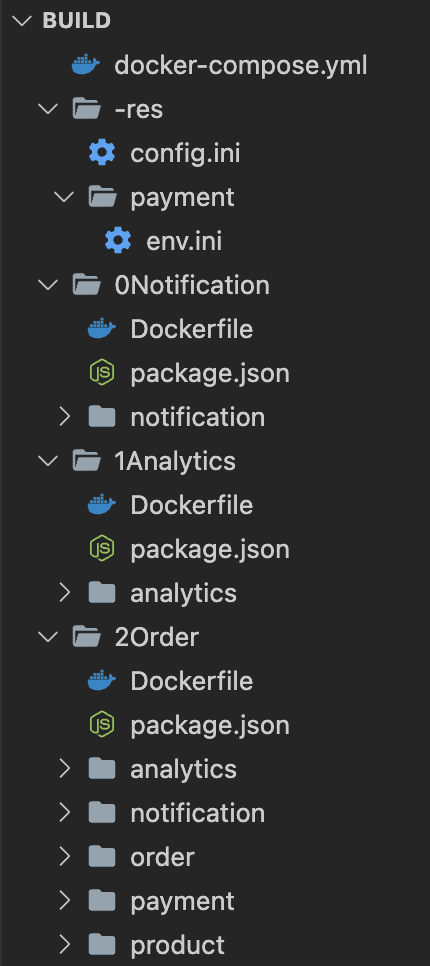
\includegraphics[width=0.35\textwidth]{figures/bf_p1.png}
    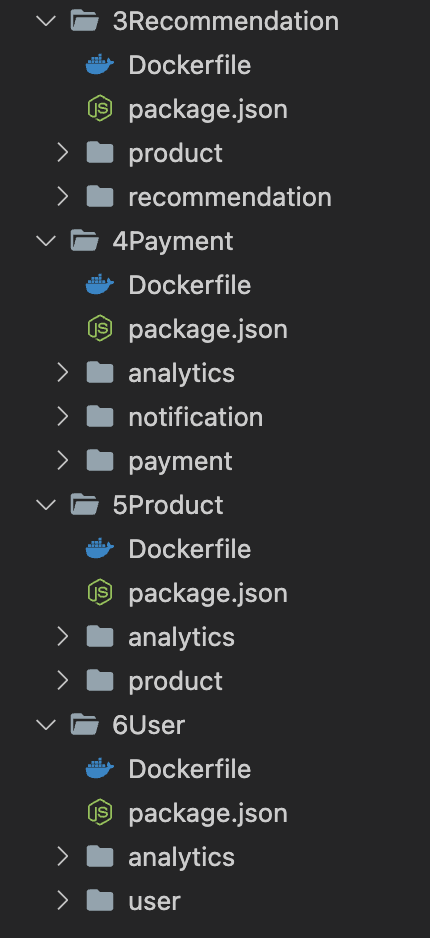
\includegraphics[width=0.35\textwidth]{figures/bf_p2.png}
    \caption{The structure of the build folders used in prototyping from the example in Chapter 3. It shows how the file structure is preserved for each service to maintain import paths. For binding volumes, the relative path to the architecture file is also maintained.}
    \label{figure:buildfolder_structure}
\end{figure}